\documentclass[sigconf, 10pt]{acmart}

\usepackage[english]{babel}
\usepackage{blindtext}
\usepackage[leqno]{amsmath}
%\usepackage{amsmath}
%\usepackage{algorithmic}
\usepackage[ruled]{algorithm2e}
\usepackage{array}
\usepackage{url}
\usepackage{epstopdf}
\usepackage{graphicx}
\usepackage{multirow}
\usepackage{subfigure}
\usepackage{multicol}
\usepackage{tabu}
\usepackage{listings}
\usepackage{makecell}
\usepackage{romannum}
\usepackage{enumerate}
\usepackage{array}
\usepackage{color}
\usepackage{booktabs}
\usepackage{threeparttable}
\usepackage{subfigure}
\usepackage{upgreek}
\usepackage{xcolor}
\usepackage{longtable}
\usepackage{bm}
% Copyright
\renewcommand\footnotetextcopyrightpermission[1]{} % removes footnote with conference info
\setcopyright{none}
\theoremstyle{plain}
\newtheorem{thm}{Theorem}[section]
\newtheorem{lem}[thm]{Lemma}
\newtheorem{prop}[thm]{Proposition}
\newtheorem{cor}{Corollary}


\settopmatter{printacmref=false, printccs=false, printfolios=true}
\acmConference[]{ICNP}{ICNP}{2018}

\begin{document}
\title{A Technique Report for KeySight}

%\titlenote{Produces the permission block, and copyright information}
\subtitle{For ICNP 2018 Submission}

% \author{Firstname Lastname}
% \authornote{Note}
% \orcid{1234-5678-9012}
% \affiliation{%
%   \institution{Affiliation}
%   \streetaddress{Address}
%   \city{City} 
%   \state{State} 
%   \postcode{Zipcode}
% }
% \email{email@domain.com}

% The default list of authors is too long for headers}
\renewcommand{\shortauthors}{Anonymous Authors}
\newcommand{\start}[1]{\vspace{5pt}\noindent\textbf{#1}}
\newcommand{\ie}{\emph{i.e.,}}
\newcommand{\eg}{\emph{e.g.,}}
\newcommand{\etal}{\emph{et al.}\xspace}

\maketitle

% \title{A Technique Report for KeySight}

\section{Introduction}

In this technique report, we will present technical materials including proof, algorithm analysis, and detailed evaluation results for KeySight which is submitted to KeySight submitted for ICNP 2018.

% This is a lits of what are presented by this paper.

% \begin{itemize}
% \item \textbf{Analysis of P4 program}
% \item \textbf{Analysis of Field Replication Algorithm}
% \item \textbf{Analysis of }
% \end{itemize}


\section{Analysis of P4 Specifiction}
We analyze P4 \cite{p4} language in term of primitive actions and special components. As there is no rigorous model for P4 language, we conduct this analysis through inference of the descriptions in P4 specification. This analysis partially answers what KeySight can see and verify at runtime. More specially, this analysis is the basis of KeyAnalyzer. The analysis result of P4 primitive actions is shown in Table \ref{tbl:primitive-actions}.

% And we can treat the new header as a parsed header outputted by the parser. Note that we should also record the validity of the new header, but we do not need to record the other fields in the new header unless the fields are read or written by in the remaining part of the P4 programs.
To record replicated filed and some spacial fields that are not explicitly declared in P4 programs. We create a new metadata called $keysight\_metadata$ to store some particular fields, and we will specify which fields will be included according to the following analysis.


\subsection{P4 Primitive Actions}
We thoroughly analysis all primitive actions supplied by P4, and conclude inputs fields and output fields in Table \ref{tbl:primitive-actions}. We categorize those primitive actions into Header Modification Actions, Field Modification Actions, Stateful Component Actions, and Forwarding-Related Actions. Furthermore, the principle and rationale of our judgment about whether a primitive action can be fully supported is also presented. In the remaining part of this section, we will respectively investigate these primitive actions. 


\begin{table*}[!tbp]
\small
\centering
\caption{Summery of P4 primitive actions.}
\label{tbl:primitive-actions}
\begin{tabular} 
{|m{0.3\linewidth}|m{0.28\linewidth}|m{0.12\linewidth}|m{0.12\linewidth}|m{0.11\linewidth}|}
%{|m{0.18\linewidth}|m{0.3\linewidth}|m{0.13\linewidth}|m{0.13\linewidth}|m{0.13\linewidth}|}
\hline
\textbf{Primitive actions} & \textbf{Descriptions from P4 Spec} & \textbf{Input fields} & \textbf{Output Fields} & \textbf{Full Support} \\
\hline
\hline
 \textit{\textbf{add\_header (hdr)}} & Add a new header into the original header stack &  & hdr\_valid & Y \\
\hline
 \textbf{\textit{copy\_header (hdr)}} & Copy one header instance to another &  & hdr\_valid & Y \\
\hline
 \textit{\textbf{remove\_header (hdr)}} & Pop the indicated header from the stack & & hdr\_valid & \\
\hline
 \textit{\textbf{modify\_field (dest, src)}} & As its name & src & dest & Y \\
\hline
 \textbf{\textit{add\_to\_field (dest, src)}} & Add a value to a field & src, dest & dest & Y \\
\hline
 \textbf{\textit{add (dest, value1, value2)}} & Add value1 and value2 and store in dest & value1, value2 & dest & Y \\
\hline
 \textit{\textbf{subtract\_from\_field (dest, value)}} & Subtract a value from a field & dest & dest & Y \\
\hline
 \textit{\textbf{subtract (dest, value1, value2)}} & Subtract value2 from value1 and store in dest & value1, value2 & dest & Y \\
\hline
 \textit{\textbf{modify\_field\_with\_hash\_based\_offset (dest, base, field\_list\_calc, size)}} & Apply a field list calculation to compute a hash value & fields in the calculation field list & dest & Y \\
\hline
 \textit{\textbf{modify\_field\_rng\_uniform {\color{white} XXXXX} (dest, lower\_bound, upper\_bound)}} & Generate a random integer number from a given range & lower\_bound, upper\_bound & dest & Y \\
\hline
 \textit{\textbf{bit\_and (dest, value1, value2)}} & Compute a bitwise AND of two values & value1, value2 & dest & Y \\
\hline
 \textit{\textbf{bit\_or(dest, value1, value2)}} & Compute a bitwise OR of two values& value1, value2 & dest & Y \\
\hline
 \textit{\textbf{bit\_xor (dest, value1, value2)}} & Compute a bitwise XOR of two values & value1, value2 & dest & Y \\
\hline
\textit{\textbf{shift\_left (dest, value1, value2)}} & Bitwise shift left & value1, value2 & dest & Y \\
\hline
\textit{\textbf{shift\_right (dest, value1, value2)}} & Bitwise shift right & value1, value2 & dest & Y \\
\hline
\textit{\textbf{truncate (length)}} & Truncate the packet on egress & length & & Y \\
\hline
 \textit{\textbf{drop ()}} & Drop the packet on egress & & egress\_port & Y \\
\hline
 \textit{\textbf{no\_op ()}} & No operation & & & Y \\
\hline
 \textbf{\textit{push (array, count)}} & Push all header instances in an array down and add a new header at the top & count & & N \\
\hline
 \textbf{\textit{pop (array, count)}} & Pop header instances from the top of an array, moving subsequent elements up & count & & N \\
\hline
 \textbf{\textit{count (counter\_ref, index)}} & Update a counter & index &  & N \\
\hline
 \textbf{\textit{execute\_meter (meter\_ref, index, field)}} & Execute a meter operation & index & field  & N \\
\hline
\textbf{\textit{generate\_digest (receiver, field\_list)}} & Generate a digest of a packet and send to a receiver & receiver &  & N \\
\hline
\textbf{\textit{register\_read (dest, register\_ref, index)}} & Read from a register & index & dest & Y \\
\hline
\textbf{\textit{register\_write (register\_ref, index, value)}} & Write to a register & index & dest & Y \\
\hline
\textbf{\textit{resubmit (field\_list)}} & Applied in the ingress pipeline, mark the packet to be resubmitted to the parser &  & resubmit\_flag & Y \\
\hline
\textbf{\textit{recirculate (field\_list)}} & On egress, mark the packet to be resubmitted to the parser &  & recirculate\_flag & Y \\
\hline
\textbf{\textit{clone\_ingress\_packet\_to\_ingress (clone\_spec, field\_list)}} & Generate a copy of the original packet and submit it to the ingress parser & clone\_spec & clone\_flag & Y \\
\hline
\textbf{\textit{clone\_egress\_packet\_to\_ingress (clone\_spec, field\_list)}} & Generate a duplicate of the egress packet and submit it to the parser & clone\_spec & clone\_flag & Y \\
\hline
\textbf{\textit{clone\_ingress\_packet\_to\_egress (clone\_spec, field\_list)}} & Generate a copy of the original packet and submit it to the Buffering Mechanism & clone\_spec & clone\_flag & Y \\
\hline
\textbf{\textit{clone\_egress\_packet\_to\_egress (clone\_spec, field\_list)}} & Duplicate the egress version of the packet and submit it to the Buffering Mechanism & clone\_spec & clone\_flag & Y \\
\hline
\end{tabular}
\end{table*}



\start{add\_header(hdr)}: This primitive action is to add a new header into a packet, and the fields in the header will be initialized to be zero. Further, $valid(hdr)$ will return true. As there is no field that records the validity of the $hdr$, we create a field called $hdr\_valid$ (1 bit) in $keysight\_metadata$. But the other fields in $hdr$ do not need to be recorded unless there are other reading or writing operations on these fields. Take $add\_header(vlan)$ as an example, we will add a new field $vlan\_valid$ in $keysight\_metadata$.  

\start{copy\_header(hdr)}: This primitive action is to add  a header and copy an old header to the new header. And we can treat the new header as a parsed header outputted by the parser. Note that we should also record the validity of the new header, but we do not need to record the other fields in the new header unless the fields are read or written by in the remaining part of the P4 programs.

\start{remove\_header(hdr)}: This primitive action is to remove a header from a packet. Just like \textit{add\_header(hdr)}, we create a field $hdr\_valid$ to record this primitive. For this primitive, the $hdr\_valid$ will be set to zero.

\start{modify\_field(dest, src)}: This primitive action is to modify a field in the metadata or packet header with a value from the packet header, metadata, action parameters, or constants. Obviously, the output field of this primitive is $dest$, while the input of this primitive is $src$. An exception is that, when $src$ is a constant or action parameter, we should not treat it as an input field as their values are recorded by $dest$.  

\start{add\_to\_field(dest, src) \& subtract\_from\_field(dest, src)}: This primitive action is to add/subtract a value $src$ to a field $dest$, \ie{} $dest = dest + src$. According to this equation, $dest$ can be viewed as the input field as well as the output field of this primitive. Further, if $src$ is not a constant or an action parameter, $src$ can also be viewed as an input field.

\start{add(dest, value1, value2) \& subtract(dest, value1, value2)}: This primitive action is to modify a field $dest$ with the sum/difference of two values $value1$ and $value2$, \ie{} $dest = value1 + value2$. According to this equation, $dest$ can be viewed as the output field of this primitive. Further, if $value1$ and $value2$ are not constants or action parameters, they can also be viewed as input fields.

\start{modify\_field\_with\_hash\_based\_offset (dest, base, field\_list\_calc, size)}: This primitive action is to modify a field through conducting a hash function on a list of fields. $dest$ can be viewed as the input field of this primitive action, while the fields that are Hashed can be viewed as the input fields.

\start{modify\_field\_rng\_uniform (dest, lower\_bound, upper\_bound)}: This primitive action is to modify a field $dest$ with a random value, \ie{} $dest = random(lower\_bound, upper\_bound)$. If $lower\_bound$ and $upper\_bound$ are not constants or action parameters, they can also be viewed input fields.

\start{bit\_and (dest, value1, value2) \& bit\_or (dest, value1, value2) \& bit\_xor (dest, value1, value2)}: These primitives conduct bitwise operations. $dest$ is the output field of this primitive. And if $value1$ and $value2$ are not constants or action parameters, they can also be viewed as input fields.

\start{ shift\_right (dest, value1, value2) \&  shift\_left (dest, value1, value2)}: These primitives conduct bit shifting operations. $dest$ is the output field of this primitive. And if $value1$ and $value2$ are not constants or action parameters, they can also be viewed as input fields.



\start{truncate (length)}: This primitive action is to cut down the number of bytes in a packet as specified by $length$. So for this action, the input field is $length$, and we create a field called $packet\_length$ (16 bits) in $keysight_metadata$ to store this value.

\start{drop ()}: This primitive action is to drop a packet. Further, this action uses different mechanisms to drop packets at the ingress pipeline and the egress pipeline. In the ingress pipeline, the P4 target drops packets through modifying the egress port of a packet to a special value, such as 255 in BMv2 \cite{bmv2-P4}. Then, in the egress pipeline, the P4 target will set a special flag to drop packets. Thus for this action, we should use different fields to denote its output field. We should use $standard\_metadata.egress\_spec$ as the output field when this action is invoked in the ingress pipeline, while we should create a new field called $egress\_drop\_flag$ (1 bit) in $keysight\_metadata$  when this action is invoked at the egress pipeline.
% So for this action, the input field is $length$, and we create a field called $packet\_length$ in $keysight_metadata$ to store this value.

\start{no\_op ()}: This primitive action has no effect on packets, thus it has no input field and output field.

\start{push (array, count) \& pop (array, count)}: These two actions add or remove packet headers from the packet stack, such as the MPLS packet stack. As $count$ various, we can not record the header validity as $add\_header$, thud we cannot model the output fields oof these actions. But we can use create a new field for $count$ to record how many headers are added or removed from the header stack. Take $push(mpls, 1)$ as an example, then we add a field called $mpls\_count$ in $keysight\_metadata$.

\start{count (counter\_ref, index)}: This primitive action is used to explicitly count the number of packets or the bytes of packets. We can only record which counter is referred by this packet through $index$, but we could know the exact counter value as the counter value is concealed from P4 programs. We should create a new field to store the counter index. Take $count(byte\_counter, 1)$ as an example, and we should create a field called $byte\_counter\_index$ in $keysight\_metadata$.

\start{execute\_meter (meter\_ref, index, field)}: This primitive action is used to execute a meter over the traffic. Just like $count (counter\_ref, index)$, we should create the index field to act as the input field. Further, this action outputs the color of the meter through $field$ which can be used as the output field. Take $execute\_meter (byte\_meter, 1, meter.color)$ as an example. We should create a new field $byte\_meter\_index$ in $keysight\_metadata$ and use this field as the input field of this primitive action. Then, $meter.color$ should be used for the output field.

\start{generate\_digest (receiver, field\_list)}: This action is to generate a message to the switch CPU, and the input field of this action is $receiver$ (if it is not a constant or a action parameter), as $field\_list$ does not impact the packet processing behavior.

\start{resubmit(field\_list) \& recirculate(field\_list)} : These primitive actions will resubmit packets into the ingress pipeline from the end of the ingress pipeline ($resubmit$) or the egress pipeline ($recirculate$). These actions will set a resubmitting flag to redirect packets. Then we can record this resubmit flag with a new field in $keysight\_metadata$.

\start{clone\_egress\_packet\_to\_egress (clone\_spec, field\_list) \& clone\_ingress\_packet\_to\_egress (clone\_spec, field\_list)} : These actions clone packets into the egress pipeline or the ingress pipeline. The cloned packets are viewed as new packets in KeySight. So we can just record whether the current packet are cloned with new fields $clone\_ingress\_flag$ and $clone\_egress\_flag$ in $keysight\_metadata$.

\subsection{Analysis of Other Components}


\start{Hash value generator}: In P4, there is a powerful method, namely field list calculation, to execute the hash value generation to satisfy various requirements, such as checksum calculation and attaining hash values. For those elements employing \textit{field list calculation}, KeyAnalyzer can take the field list in the calculation declaration. Then, the output field of field list calculation is determined by the invoked primitive actions. 

\start{Action profile}: This component supports selecting executed action based on hash values (attained from the hash value generator) and can be applied to implement ECMP. This component can be also modeled by KeyAnalyzer, as KeyAnalyzer can fully analyze all the actions in a match action table and can identify inputs as well as outputs of each action. Thus, KeyAnalyzer does not require explicit identification of which action should be executed by a table entry and can support such a situation where the action to be executed is determined dynamically by packet header fields. 





\section{Filed Replication Algorithm}


% \section{Survey of P4 Applications}



\subsection{Time and Space Complexity}
We evaluate the run-time complexity for the worst-case scenario of the field replication algorithm by examining the structure of the algorithm and making some simplifying assumptions.

In the algorithm, KS denotes the key structure, V denotes the processing unit set and E denotes the control flow sequence. In our research, we assume the graph is a DAG. $O_{v}$,  $O^{c}_{v}$, $R_{v}$, $R^{a}_{v}$, $I_{v}$ respectively represent the output of the vertex v, the copy of output of the vertex v, the replication of output of the vertex v, the pending replication of output of the vertex v and the input of the vertex v.

Actually, we have omitted the part where we initialize the sets which include $O_{v}$,  $O^{c}_{v}$, $R_{v}$, $R^{a}_{v}$, $I_{v}$ as empty sets in Algorithm 1. We denote K as the maximum of the numbers of possible values for each domain, $|V|$ as the amount of vertexes and $|E|$ as that of edges. Further, we use F to denote a set of all field in headers and metadata of a P4 program, thus $|F|$ is the number of fields. Besides that, we mark each line with a number in order to illustrate the time and space complexity conveniently.

Say that the actions carried out in line 1 are considered to consume time T1, line 2 uses time T2, and so forth.
In the algorithm above, lines 1, 2, 14 will only be run once. Thus the total amount of time to run lines 1, 2 and 14 is:
$ T_{1}+T_{2}+T_{14}.$ Apparently, $ T_{1} = O(1)$. For line 2, since the number of edges and vertexes are generally limited in our P4 programs, we can use the Kahn algorithm to accomplish the topological sort and thus $ T_{2} = O(|V| + |E|)$. As for line 14, the union process is executed scanning every domain of $R^{a}_{v}$ and the corresponding domain of $KS$, therefore $ T_{14} = O(|F|)$.

To estimate the complexity of For loop more accurately, we can divide it as two parts: lines 4-9 and lines 10-15, the latter of which is simpler to understand.

Considering the number of domains in P4 programs are usually limited, we can use hash tables to implement the union, intersection, and subtraction operation of sets without collision and we just need to scan the two sets to build the specific hash tables. In conclusion, we can achieve the operations in lines 10-14 with the time complexity $O(M)$ and the total time consumption $T_{10} + T_{11} + T_{12} + T_{13} + T_{14}$ equals to $O( |V||F| + 3|V||F| + 3|V||F| + |V|+|F|)$, that is $O(|V||F| + |V|)$, because lines 10-13 are executed for each vertex in the graph.


For lines 4-9, we could find it that the traversals of all the children of vertices actually need $O(E)$ time since the most inner operations will be executed for each edge. Mentioning that the union, intersection, and subtraction operation of sets can be finished in $O(M)$ time, the time complexity of lines 4-9 is $T_{4} + T_{5} + T_{6} + T_{7} + T_{8} + T_{9}$ is $O(|E||F|)$.

Therefore 
\begin{displaymath}
\sum_{i=1}^{17}T_{i}= O(|V|+|E|+|F|+|V||F|+|E||F|) =O(|F|(|V|+|E|))
\end{displaymath}


As for space complexity, each vertex has sets of input, output, pending replication and replication, all of which consume $O(|F|K)$ space. In total, the space consumption is O(|V||F|K). Apart from that, KS requires space of $O(|F|K)$ complexity and the initial adjacency list for the control flow graph demands $(|V|+|E|)$ space. So the total space complexity is $O(|V||F|K+|E|)$.

\begin{algorithm}[!t]
\LinesNumbered
\KwIn{A control flow graph G = (V, E)}
\KwOut{A PEC representation (\textit{pec})}
$pec \leftarrow \emptyset$ \;
$ V^{*} \leftarrow $ Reverse(TopologicalSort(V, E)) \;
\ForEach{$v$ in $V^{*}$} {
    \ForEach{child vertex $v'$ of $v$} {
    	$O^c_v \leftarrow O^c_v \cup O^c_{v'}$ \;
    	$ R_v \leftarrow R_v \cup ( O_v \cap O^c_{v'} ) $ \;
    	$ R_v \leftarrow R_v \cup ( O_v \cap R_{v'}^a )$ \;
        $ R^a_v \leftarrow R^a_v \cup R^a_{v'}  $ \;
    }    
	$O^c_v \leftarrow O^c_v \cup O_v $ \;
    $R^a_v \leftarrow (R^a_v \setminus R_v) \cup (I_v \cap O^c_v) $ \;
    \textit{pec} $\leftarrow$ \textit{pec} $ \cup \ O_v \cup I_v \cup \{r|\ \text{\textit{$r$ is a replica of $x$}}, x \in R_v\} $\;
    \If{$v$ is the last of $V^*$} {
    	\textit{pec} $\leftarrow$ \textit{pec} $ \cup \ \{r|\ \text{\textit{$r$ is a replica of $x$}}, x \in R^a_v\}  $\;
    }
}
\KwRet{pec}\;
\caption{Field Replica Algorithm}
\label{alg:field-replica}
\end{algorithm}

% \section{Analysis of Streaming Bloom Filter}

% The fraction of 1 every window is $\rho$. And we can get it from the following equation.

% $$
% \rho = \frac{(1 - \frac{1}{M})^N}{1 + (1 - \frac{1}{M \times B})^N}
% $$


\subsection{Network-wide PEC Definition}

In this section, we first present a network-wide PEC definition. 

\noindent\textsl{\textbf{Definition (Network-wide Packet Equivalence Class)}}: In a network, 
a Network-wide Packet Equivalence Class is a set $\mathcal{C}$ of packets such that any packet $pkt_1, pkt_2 \in \mathcal{C}$ has following properties:

\begin{itemize}
    
    \item $pkt_1$ and $pkt_2$ traverse the same programmable switches in the same order, and those switches compose a forwarding path;
    \item In each switch of the forwarding path, $pkt_1$ and $pkt_2$ traverse the same MATs, and those MATs compose a MAT set;
    \item For each MAT in the MAT set, $pkt_1$ and $pkt_2$ hit the identical MAT entry whose compound action is $\mathcal{A}$;
    \item For each primitive action invoked in $\mathcal{A}$, $pkt_1$ and $pkt_2$ have the same inputs and outputs.

\end{itemize}


\subsection{Proof for KeyAnalyzer}

In this section, we will show the proof for KeyAnalyzer. First, we present the proof for field replication algorithm (FRA). Then, based on the proof of FRA, we present the proof for KeyAnalyzer.

As for the FRA, it can satisfy the following corollary.

\begin{cor}

    The PEC representations generated by FRA can identify that inputs and outputs of every table in P4 programs without conflicts.

\end{cor}
    
    
\begin{proof}
    As be analyzed in the paper, the reversed-match dependency and the action dependency makes the input fields and output fields of some tables overlap. 
    Satisfying above corollary, FRA is to remove these two dependencies in essence. So we need to prove how FRA correctly remove the dependencies.
    It is evident that in FRA, when processing a table, the children of this table have been processed, which is ensured by the reversed topological sort algorithm. Besides, the two dependencies happen when a field is written in the ancestor, 
    while its children read or write the same field. Based on the above statements, 
    we can use loop invariants to illustrate why FRA can exactly attain input fields and output fields of every table.
    
    \start{Initialization}: At the beginning, $pec$ does not store the input fields and output fields for any table. 
    Thus, it is true for FRA to keep the property that $pec$ stores inputs fields and output fields of every table. 
    
    \start{Maintaince}: We assume that the property of $pec$ is true before processing $v$. Then, for $v$, all its children have be processed. 
    Then, for every children, FRA will find the fields that trigger action dependency (line 6) and reversed-match dependency (line 11). FRA will create replications for these fields to record them. 
    The replication fields, input fields, and output fields are added into $pec$. Thus, for $v$, $pec$ can record input fields and output fields correctly. 
    
    \start{Termination}: When $v$ is the last one in $V*$, input fields and output fields of all children of $v$ and $v$ are stored in $pec$. 
    Further, there are some pending replication fields that should be replicated with an additional table at the start of P4 pipeline. 
    Then, $pec$ can store input fields and output fields of every table in P4 programs.
\end{proof}
    


Based on the above analysis, we can state that KeyAnalyzer can satisfy the following corollary.

\begin{cor}

The PEC representation extracted by KeyAnalyzer guarantees that for any packet $pkt_1$ and $pkt_2$, they belong to a PEC if and only if postcard $p_1$ of $pkt_1$ equals to postcard $p_2$ of $pkt_2$.

\end{cor}


\begin{proof}
    % First of all, KeyAnalyzer conducts action-level analysis on P4 programs, then it can get input fields and output fields of every primitive action. 
    FRA guarantees that input fields and output fields of every MAT is recorded, then \textbf{$\bm{\mathcal{P}_1}$} can be satisfied, as the inputs and outputs can also identify the traversed MATs. Further, the MAT-level analysis guarantees that only two packets hit the same table entry in the same MAT, they can have the same output or inputs.
    Further, the action-level analysis helps ensure that PECs correctly record inputs and outputs of every primitive actions.

\end{proof}

\section{Ring Bloom Filter}

\newcommand{\Y}{{\color{red}$\checkmark$}}
\newcommand{\N}{{\color{green}\textbf{$\times$}}}

In this section, we will introduce the theoretical analysis of Ring Bloom Filter (RBF) shown in Figure \ref{fig:rbf-parameter}, including false negative rates (FNR) and false positive rates (FPR). 
To be intuitive, we firstly demonstrate the parameters of RBF, then we will present FPRs and FNRs of SBF in terms of recently-arrived packets. At last, we will show how to tune RBF to attain different FNRs and FPRs.

\begin{figure*}[!htbp]
\centering
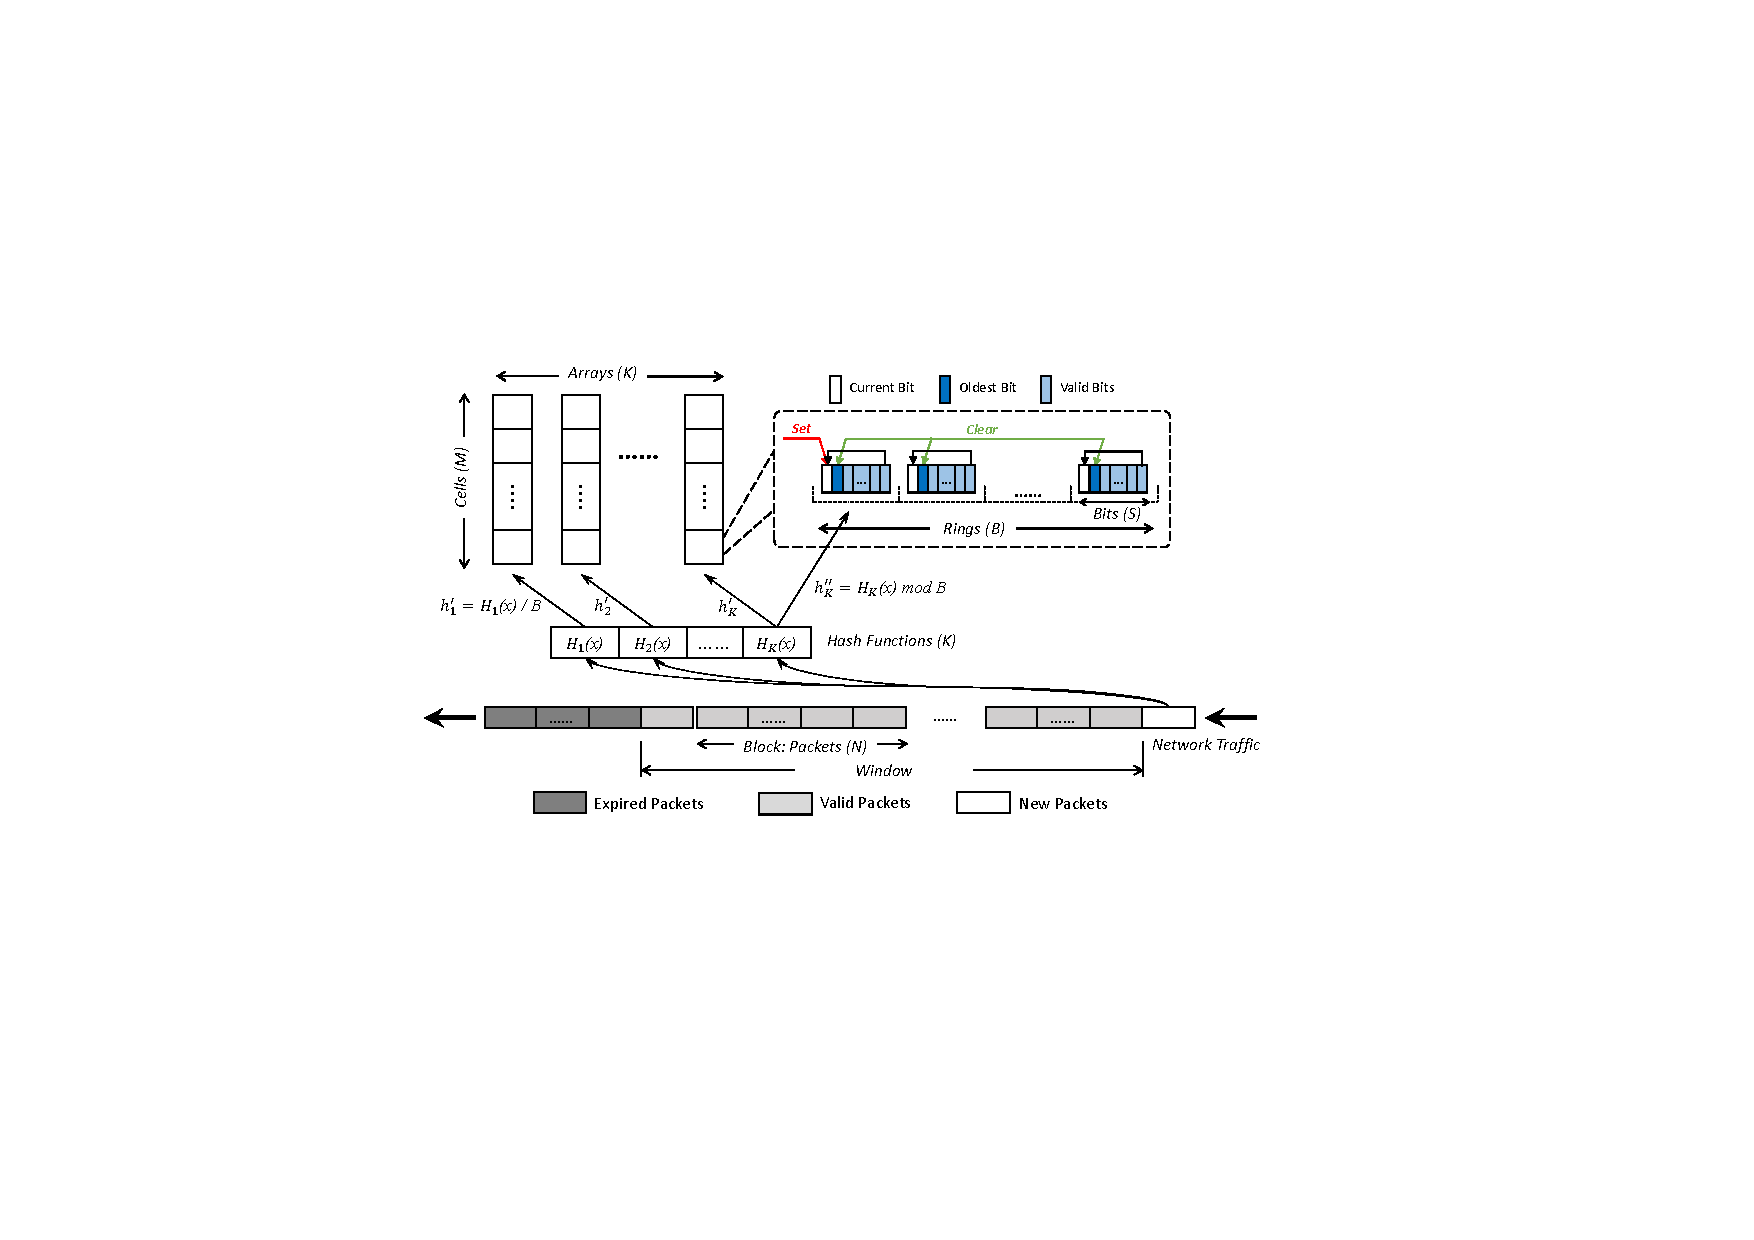
\includegraphics[width=0.9\textwidth]{graphs/rbf.pdf}
\caption{Architecture overview of Ring Bloom Filter.} 
\label{fig:evaluation}

\end{figure*}


\subsection{Parameters of RBF}

In this section, we briefly introduce parameters of RBF as well as their meanings.


Bloom Filter Queue (BFQ) could have multiple ($S$) bloom filters (BF) with single-bit cells, while the other algorithms only have one bloom filter. Inside one BF, there could be several arrays, each of which has M cells. For BSBF, BSBFSD, RLBSBF, and BFQ, a cell has one bit, while RBF and SBF can have multiple bits per cell.
Specifically, in a cell, RBF have B rings, each of which has S bits because the BFs in BFQ are merged into one BF in RBF. Unlike the other algorithms, BFQ and RBF have a parameter that denotes how many packets in a block, and the number of recently-arrived packets is $N \times (S - 1)$.
Besides, the number of bits per ring and the number of rings per cell as well as the block size can be dynamically reconfigured at runtime, which provides much flexibility for operators to tune RBF.
Further, RBF can have closer attributes to BFQ when $B$ becomes larger,

\begin{table*}
\caption{Notation Summery of SBF and RBF. \Y{} denotes that this parameter can be dynamically adjusted in run time, while \N{} denotes this parameter is fixed in run time.}
\label{fig:rbf-parameter}
\small
\begin{tabular}{|m{0.08\linewidth}|m{0.25\linewidth}|m{0.18\linewidth}|m{0.09\linewidth}|m{0.09\linewidth}|m{0.09\linewidth}|m{0.09\linewidth}|}

\hline
\textbf{Notations} & \textbf{Description} & \textbf{BSBF/BSBFSD/RLBSBF} & \textbf{SBF} & \textbf{BFQ} & \textbf{RBF} & \textbf{Reconfig.} \\
\hline
\hline

$S$ & \# of BFs & 1 & 1 & $>1$ & 1 & \N \\
\hline
$K$ & \# of Arrays per BF & $>1$ & $>1$ & $>1$ & $>1$ & \N \\ 
\hline
 & \# of Bits per Array & $M$ & $M \times Max $ & $M$ & $M \times B \times S$ & \N \\
\hline
$A$ & \# of Bits per Cell & 1 & $Max$ & 1  & $B \times S$ & \N \\ 
\hline
$B$ & \# of Rings per Cell & - & - & - & $>1$ & \Y \\ 
\hline
$S$ & \# of Bits per Ring & - & - & - & $>1$ & \Y \\ 
\hline
$M$ & \# of Cells per Array  & $>1$ & $>1$ & $>1$ & $>1$ & \Y \\ 
\hline
$N$ & \# of Packets per Block  & - & - & $>1$ & $>1$ & \Y \\ 
\hline
& \# of Recently-arrived Packets  & - & - & $N \times (S - 1)$ &$N \times (S - 1)$ & \Y \\
\hline
& \# of Total Bits  & $M \times K$ & $M \times K \times Max$ & $M \times K \times S$ &$M \times K \times S \times B$ & \N \\
\hline
\end{tabular}

\end{table*}

\subsection{Analysis of RBF}


In this section, we will present an analysis on the FNR and the FPR of BFQ, because RBF has similar attributes to BFQ. Then we will present our experience on tuning RBF.

For Bloom Filter, the false positive rate (FPR) is:
\begin{equation}
    \left( 1 - \left(1-  \frac{1}{M}\right)^{N} \right) ^ K
\end{equation}

And the false negative rate (FNR) of Bloom Filter is 0.

For Bloom Filter Queue, the false positive rate of the recently-arrived packets is:
\begin{equation}
    \left( 1 - \left(1-  \frac{1}{M}\right)^{N(S-1)} \right) ^ K
\end{equation}

And the FNR of BFQ when only considering recently-arrived packets is 0.

For all the packets in the network traffic, FNR of BFQ depends on the flow length, i.e., how many packets in the same flow. 
So if $N$ is too small, the FNR of BFQ will become very large, but the FPR will be pretty small. Further, $S$ has the similar effects on FNR and FPR with $N$, \ie{} a larger $N$ stands for better FNR but worse FPR, while a smaller $N$ stands for better FPR but worse FNR. 

\bibliographystyle{ACM-Reference-Format}
\bibliography{reference}

\end{document}